\documentclass{article}
\usepackage{tikz}
\usepackage{graphicx}  % Required for the resizebox command
\usepackage{amsmath}  % for the array environment

\usepackage{array}
\usepackage{mathpazo}

\usepackage{fullpage}

\begin{document}

\section*{Introduction}

This document presents a methodology for forecasting industrial decarbonization incentivized 
by a carbon price. The agents in our model are firms operating in various industrial sectors, 
including but not limited to producers of Iron and Steel, Cement, Plastics, and Chemicals. 
Importantly, while these are examples, the methodology is sector-agnostic and can be applied 
to other similar problems.
Central to the model is the decision-making of firms. Given a set carbon price and considering 
the age of their current facilities within a sector as well as the prevailing technological landscape, 
firms will decide whether or not to invest in green technology. It's worth noting that within each sector, 
we make the simplifying assumption that firms produce a singular, homogeneous good. For instance, 
despite the existence of myriad steel varieties—many of which are not substitutes for one another—we assume 
that all steel producers generate the same kind of steel.
\section{Model set-up}

The firm will make decision
\\
\\
\resizebox{\textwidth}{!}{%
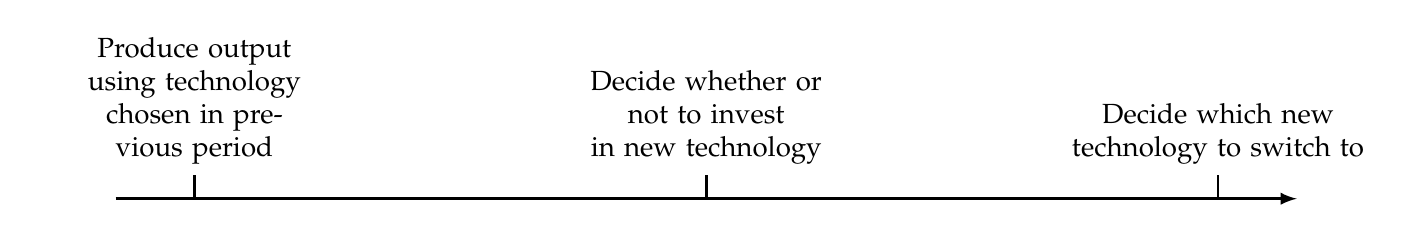
\begin{tikzpicture}[>=latex,line width=1pt]  % Setting the line width and arrow tip style
    % Draw horizontal line with an arrow at the end
    \draw[->] (0,0) -- (15,0);  % Increased the length to 15
    
    % Draw shorter vertical lines and add annotations
    \draw (1,0) -- (1,0.3) node[above, text width=4cm, align=center] {Produce output\\ using technology\\ chosen in previous period};
    \draw (7.5,0) -- (7.5,0.3) node[above, text width=4cm, align=center] {Decide whether or\\ not to invest\\ in new technology}; 
    \draw (14,0) -- (14,0.3) node[above, text width=4cm, align=center] {Decide which new\\ technology to switch to};
\end{tikzpicture}%
}
\\
\\
\subsection{Technology turnover}
In the simplest version of the model, the decision whether to invest in a new technology is made once every \( L \) periods. Where \( L \) is the lifetime of the asset in the sector.
Assets are assumed to homogeneous within a sector with respect to their lifetime. We will need to keep track of when technology switching occurs and the distribution of the age of the assets
within a sector. To this end, let us define a matrix \( \mathbf{A}^t \) where \( \mathbf{A}^t_{\theta, l} \) is the percentage of facilities in the sector using technology \( \theta \) that are \( l \) years old at time \( t \). If when 
we are able to define a stochastic matrix \( \mathbf{P}^t \) where \( \mathbf{P}^t_{\theta, \theta^{'}} \) is the probability that a firm using technology \( \theta \) in period \( t \), will switch to technology \( \theta^{'} \) in the next period, 
we can update \( \mathbf{A}^t \) as follows:
\begin{equation}
    \mathbf{A}^{t+1} = \bigg[\mathbf{P}^t \mathbf{A}^t[L] , \mathbf{A}^t[1], \ldots, \mathbf{A}^t[L-1]\bigg] 
\end{equation}
\subsection{Technology choice}

For any given sector, firms have a range of production technologies available, 
indexed by $\theta$ which spans from $1$ to $\Theta$. Each of these production technologies 
comes with its own fixed cost, $F_{\theta, t}$, which is incurred only once during the 
asset's lifetime. Additionally, there's a variable cost, $c_{\theta, t}$, and a carbon intensity, $e_{\theta, t}$. 
Therefore, when switching to a new technology, the production cost is represented by:

\begin{equation}
    C_{\theta, t} 
    = F_{\theta, t} + 
    \sum_{\tau=t}^{L}\beta^{t-\tau}(c_{\theta, \tau} + e_{\theta, \tau} \cdot p_{\tau} + \epsilon^{i}) \cdot D^{i}
\end{equation}

In the above equation, $p_t$ denotes the prevailing carbon price at time $t$, while $D_i$ refers to the demand allocated to the $i$th firm. 
Consequently, the primary objective for any firm is to select a technology, $\theta^*$, that minimizes the cost. 
This decision can be mathematically represented as:

\begin{equation}
    \theta^*_{t} = \arg\min_{\theta \in \Theta} C_{\theta, t} 
\end{equation}

Sketch of a solution (this will have to worked out in detail, however, 
I'm quite sure that given some distributional assumtion a solution 
similiar to the one below can be obtained). 
\\  
\\
Assuming $\epsilon^i \sim $ Gumbel$(-\gamma \nu,\nu)$. It can be shown that:
\begin{equation}
    \mathbf{P}[\theta^{'} = \theta^{*}] = \frac{\exp(-C_{\theta^{'}, t})^{1/\nu}}{\sum_{\theta \in \Theta}\exp(-C_{\theta, t})^{1/\nu}}
\end{equation}
Assuming a continum of firmas will get that shares of firms choosing a given $\theta^{'}$ will be approach the probabilities above. 

\subsection{Competition and demand reduction}
asdf
\section{Calibration and estimation of parameters}
\subsection{Modelling the variable cost of production}
asdf
\end{document}